\subsection{二视图}\label{subsec:czjh2-8-2}

\subsubsection{二视图的概念}

当一些物体或零件比较复杂时,只用一个正投影图很难把它的形状特征表示清楚,
这时往往需要从不同的投射方向,把物体或零件投影到两个互相垂直的投影面上,用两个正投影图来表示它们。
\begin{figure}[htbp]
    \centering
    \begin{minipage}[b]{7cm}
        \centering
        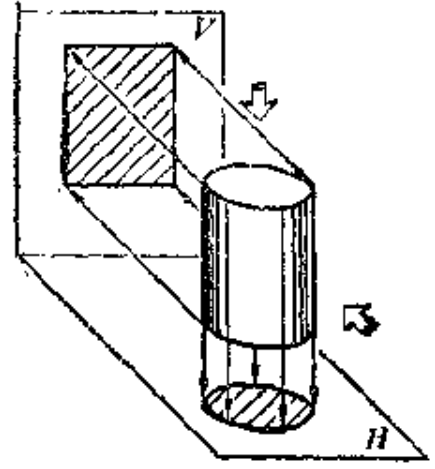
\includegraphics[width=4cm]{../pic/czjh2-ch8-07.png}
        \caption{}\label{fig:czjh2-8-7}
    \end{minipage}
    \begin{minipage}[b]{7cm}
        \centering
        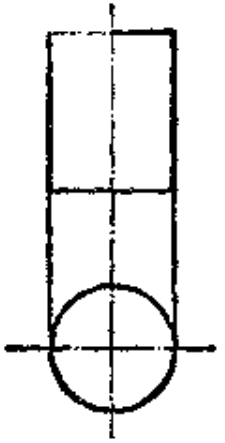
\includegraphics[width=2cm]{../pic/czjh2-ch8-08.png}
        \caption{}\label{fig:czjh2-8-8}
    \end{minipage}
\end{figure}
下面我们来看将一个圆柱放在互相垂直的两个投影面间进行正投影的情形。
如图 \ref{fig:czjh2-8-7} 所示,在正面投影面 $V$ 上的视图是一个矩形,长等于圆柱的直径,
高等于圆柱的高,在水平投影面 $H$ 上的视图是一个圆,它与圆柱的底是等圆。



将圆柱拿走,把水平投影面 $H$ 往下转 $90^\circ$,使投影面 $H$ 与 $V$ 在同一平面上,
我们就得到如图 \ref{fig:czjh2-8-8} 所示的图形。

在正面投影面 $V$ 上所得到的视图称为\zhongdian{主视图};

在水平投影面 $H$ 上所得到的视图称为\zhongdian{俯视图}。

主视图和俯视图统称为\zhongdian{二视图}。

画物体的二视图时,主视图画在上面,俯视图画在它的下面,而且两个视图要对正。
画对称形物体的视图时,要先画物体的对称轴线或中心线,用点划线表示。

现在我们以图 \ref{fig:czjh2-8-1} 中的零件上半部为例,研究这个空心圆柱的二视图。

空心圆柱的外形是圆柱,空心部分也是圆柱,所以它的俯视图是两个同心圆,它的主视图是两个矩形。
如图 \ref{fig:czjh2-8-9} 所示,圆柱的外形部分是看得见的,画粗实线;圆柱的空心部分是看不见的,画虚线。

\begin{figure}[htbp]
    \centering
    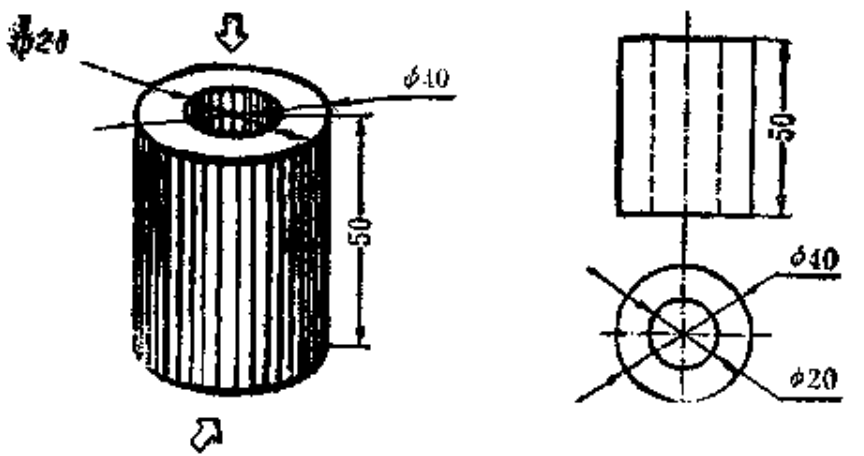
\includegraphics[width=8cm]{../pic/czjh2-ch8-09.png}
    \caption{}\label{fig:czjh2-8-9}
\end{figure}

在画视图时规定,\zhongdian{看得见部分的轮廓线画粗实线,看不见部分的轮廓线画虚线。}

每一个视图画好后,都要标注尺寸,这样便于加工。图纸上不具体注明尺寸单位的都是指 mm ,
如图 \ref{fig:czjh2-8-9},图中高 50 就是 50 mm, $\phi 40$ 就是直径为 40 mm。
图线的使用和尺寸的注法可参看本章\hyperref[sec:czjh2-8-fulu]{附录}。

二视图的画法规则可以概括为

\begin{center}
    \framebox{\zhongdian{上主下俯长对正,实线虚线要分清。}}
\end{center}


\subsubsection{二视图的画法}

以圆锥为例,如图 \ref{fig:czjh2-8-10}(a),它的二视图应该怎样画呢?
根据二视图的画法规则,圆锥的主视图是一个等腰三角形,俯视图是一个圆。
圆锥的二视图的具体画法如下:

\begin{figure}[htbp]
    \centering
    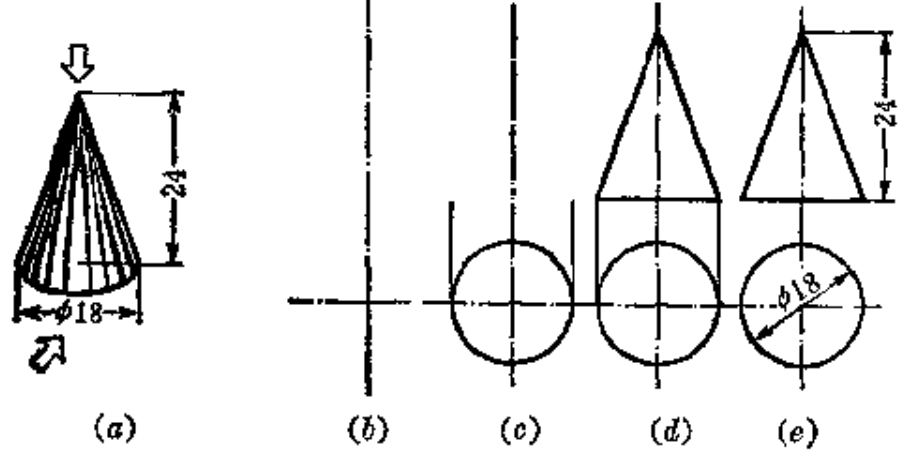
\includegraphics[width=9cm]{../pic/czjh2-ch8-10.png}
    \caption{}\label{fig:czjh2-8-10}
\end{figure}

(1)画出对称轴线 —— 点划线,如图 \ref{fig:czjh2-8-10}(b);

(2)画出俯视图,即画直径为 18 mm 的圆,如图 \ref{fig:czjh2-8-10}(c);

(3)根据主视图、俯视图上下长对正与已知圆锥的高等于 24 mm,画出等腰三角形,如图 \ref{fig:czjh2-8-10}(d);

(4)标注尺寸,擦去不必要的辅助线,如图 \ref{fig:czjh2-8-10}(e)。

再如画圆台的二视图,如图 \ref{fig:czjh2-8-11}(a),已知圆台上下两底的直径分别为 20 mm和 40 mm,高为 40 mm,
它的二视图的画法步骤与圆锥二视图的画法相同,具体画法如图 \ref{fig:czjh2-8-11}(b)、(c)、(d)、(e),由同学自己分析。

% \begin{figure}[htbp]
%     \centering
%     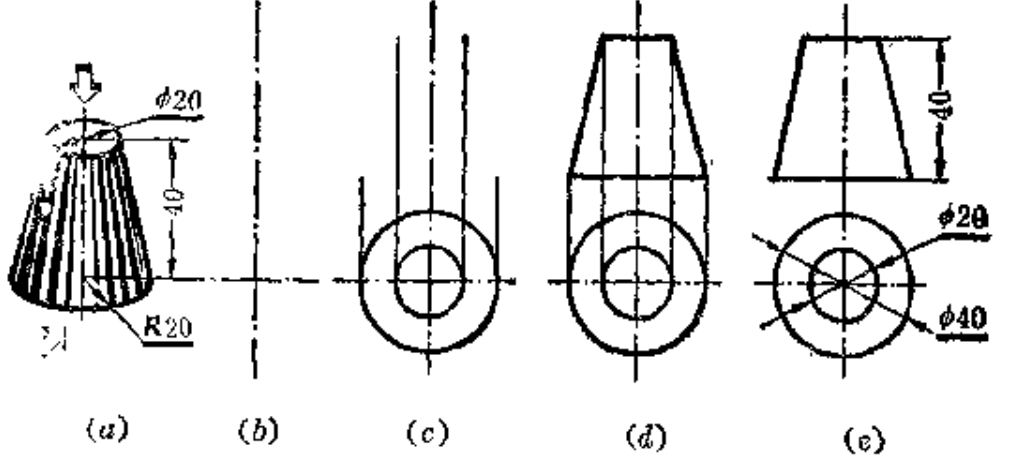
\includegraphics[width=9cm]{../pic/czjh2-ch8-11.png}
%     \caption{}\label{fig:czjh2-8-11}
% \end{figure}

画图时,可以根据实物的大小和其结构的复杂程度,用一定的比例尺进行放大或缩小。
加工零件时,以图上的尺寸数字为准。

\begin{figure}[htbp]
    \centering
    \begin{minipage}[b]{10cm}
        \centering
        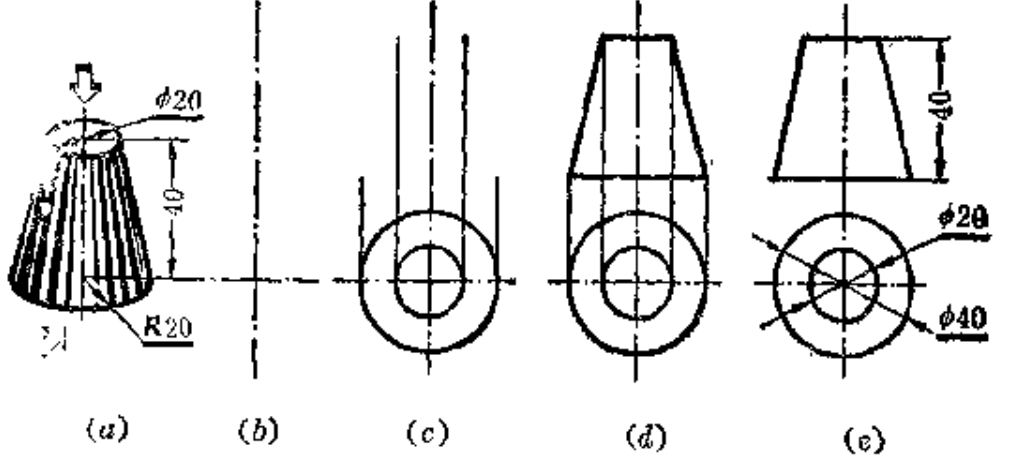
\includegraphics[width=9cm]{../pic/czjh2-ch8-11.png}
        \caption{}\label{fig:czjh2-8-11}
    \end{minipage}
    \begin{minipage}[b]{4cm}
        \centering
        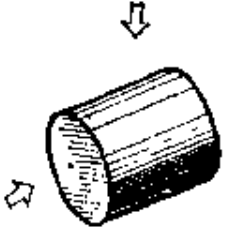
\includegraphics[width=3cm]{../pic/czjh2-ch8-subsec2-lx-01.png}
        \caption*{(第 1 题)}
    \end{minipage}
\end{figure}

\begin{lianxi}

\xiaoti{任何圆柱的主视图总是矩形,俯视图总是圆,这种说法对吗?如果圆柱按图中的放法,它的二视图是怎样的?}

\xiaoti{说出下列几何体的二视图。}

\begin{figure}[htbp]
    \centering
    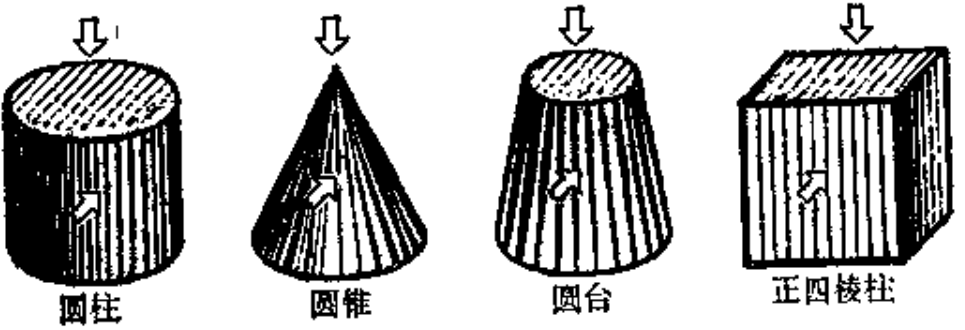
\includegraphics[width=9cm]{../pic/czjh2-ch8-subsec2-lx-02.png}
    \caption*{(第 2 题)}
\end{figure}

\xiaoti{下面是空心圆柱的二视图,哪个有错误?为什么错?}

\begin{figure}[htbp]
    \centering
    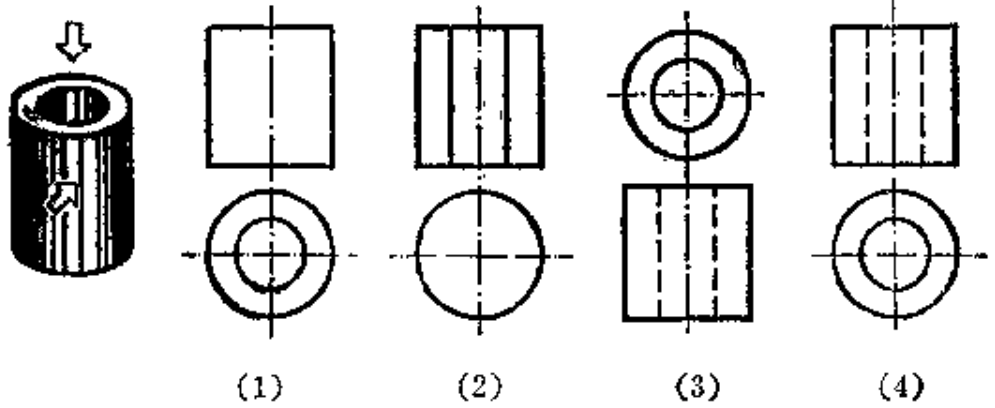
\includegraphics[width=9cm]{../pic/czjh2-ch8-subsec2-lx-03.png}
    \caption*{(第 3 题)}
\end{figure}

\end{lianxi}

